\documentclass[tikz]{standalone}
\usepackage{tikz}
\usepackage{etoolbox}
\usetikzlibrary{positioning,matrix,backgrounds}


\pgfdeclarelayer{background}
\pgfdeclarelayer{foreground}
\pgfsetlayers{background,main,foreground}

% Define the sindy component as a node style
\tikzset{
    sindy component/.style={
        rectangle,
        minimum width=0.8cm,
        minimum height=1.5cm,
        text width=0.8cm,
        text height=1.5cm,
        rounded corners=5pt,
        fill=gray,
        draw=none,
        inner sep=0pt,
        outer sep=0pt,
        align=center
    },
    sindy label/.style={font=\small, text=black},
    sindy color/.style={fill=#1},
    sindy label color/.style={label={[sindy label, text=#1]above:##1}},
    with label/.style={label={[sindy label, anchor=south]above=3mm:#1}}
}

\begin{document}
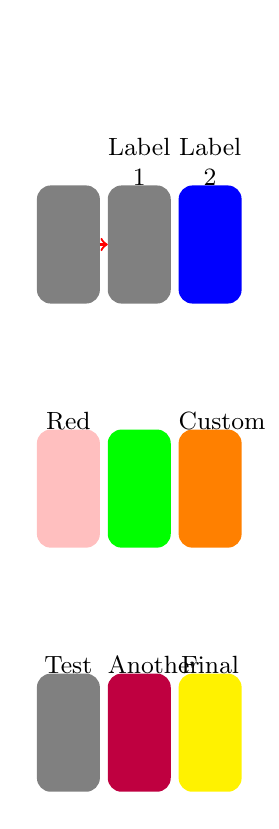
\begin{tikzpicture}

% Create a matrix of nodes with automatic naming (m-row-column)
\matrix[matrix of nodes,
        column sep=0.1cm, 
        row sep=0.1cm,
        nodes={sindy component}] (m) {
    |[fill=gray]| &
    |[fill=gray, with label=Label 1]| &
    |[fill=blue, with label=Label 2]| \\
    |[fill=pink, with label=Red]| & 
    |[fill=green]| &
    |[fill=orange, with label=Custom]| \\
    |[fill=gray, with label=Test]| &
    |[fill=purple, with label=Another]| &
    |[fill=yellow, with label=Final]| \\
};

% Example: Connect nodes using automatic names m-row-column
\draw[red, thick, ->] (m-1-1.east) -- (m-1-2.west);
% \draw[blue, thick, ->] (m-2-1.south) -- (m-3-1.north);

\end{tikzpicture}
\end{document}